\documentclass{standalone}
\usepackage{tikz}
\usetikzlibrary{patterns, positioning}
\usepackage[sfdefault]{ClearSans} %% option 'sfdefault' activates Clear Sans as the default text font
\usepackage[T1]{fontenc}

\begin{document}
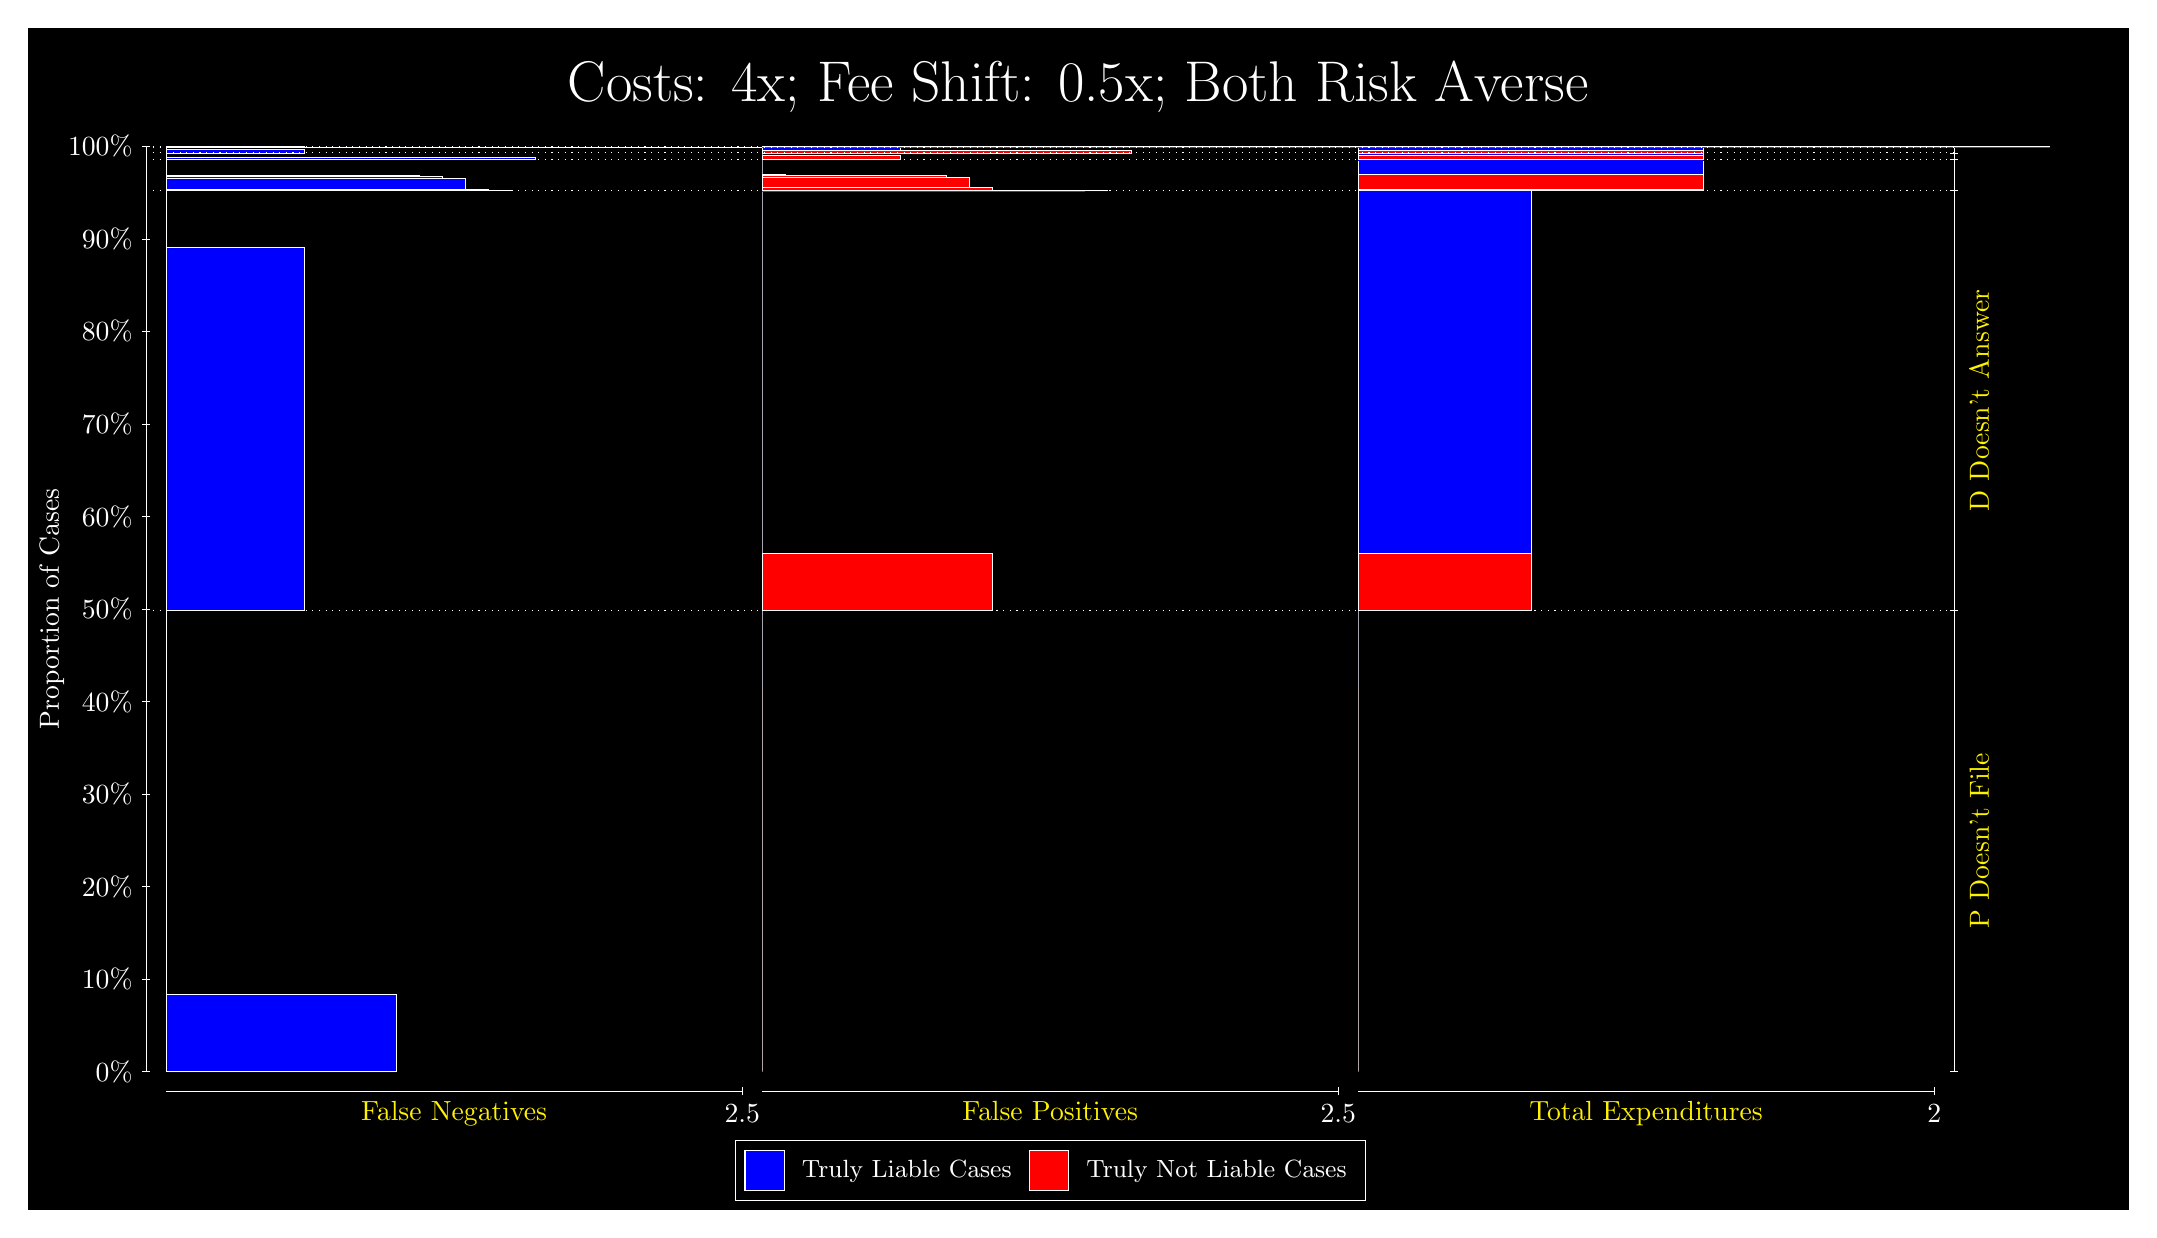
\begin{tikzpicture}
\draw[fill=black] (0,0) rectangle (26.667,15);
\draw[text=white] (0,13.5) rectangle (26.667,15) node[midway] {\huge Costs: 4x; Fee Shift: 0.5x; Both Risk Averse};
\draw[white, very thin] (1.5,1.75) -- (1.5,13.5);
\node[rotate=90, text=white, anchor=center] at (0.3, 7.625) {Proportion of Cases};
\draw[white, very thin] (1.45,1.75) -- (1.55,1.75);
\node[text=white, anchor=east] at (1.45, 1.75) {0\%};
\draw[white, very thin] (1.45,2.925) -- (1.55,2.925);
\node[text=white, anchor=east] at (1.45, 2.925) {10\%};
\draw[white, very thin] (1.45,4.1) -- (1.55,4.1);
\node[text=white, anchor=east] at (1.45, 4.1) {20\%};
\draw[white, very thin] (1.45,5.275) -- (1.55,5.275);
\node[text=white, anchor=east] at (1.45, 5.275) {30\%};
\draw[white, very thin] (1.45,6.45) -- (1.55,6.45);
\node[text=white, anchor=east] at (1.45, 6.45) {40\%};
\draw[white, very thin] (1.45,7.625) -- (1.55,7.625);
\node[text=white, anchor=east] at (1.45, 7.625) {50\%};
\draw[white, very thin] (1.45,8.8) -- (1.55,8.8);
\node[text=white, anchor=east] at (1.45, 8.8) {60\%};
\draw[white, very thin] (1.45,9.975) -- (1.55,9.975);
\node[text=white, anchor=east] at (1.45, 9.975) {70\%};
\draw[white, very thin] (1.45,11.15) -- (1.55,11.15);
\node[text=white, anchor=east] at (1.45, 11.15) {80\%};
\draw[white, very thin] (1.45,12.325) -- (1.55,12.325);
\node[text=white, anchor=east] at (1.45, 12.325) {90\%};
\draw[white, very thin] (1.45,13.5) -- (1.55,13.5);
\node[text=white, anchor=east] at (1.45, 13.5) {100\%};

\draw[white, very thin] (24.457,1.75) -- (24.457,13.5);
\draw[white, very thin] (24.407,1.75) -- (24.507,1.75);
\node[anchor=west] at (24.407, 1.75) {};
\draw[white, very thin] (24.407,7.6078) -- (24.507,7.6078);
\node[anchor=west] at (24.407, 7.6078) {};
\draw[white, very thin] (24.407,12.937) -- (24.507,12.937);
\node[anchor=west] at (24.407, 12.937) {};
\draw[white, very thin] (24.407,13.332) -- (24.507,13.332);
\node[anchor=west] at (24.407, 13.332) {};
\draw[white, very thin] (24.407,13.416) -- (24.507,13.416);
\node[anchor=west] at (24.407, 13.416) {};
\draw[white, very thin] (24.407,13.49) -- (24.507,13.49);
\node[anchor=west] at (24.407, 13.49) {};
\draw[white, very thin] (24.407,13.496) -- (24.507,13.496);
\node[anchor=west] at (24.407, 13.496) {};
\draw[white, very thin] (24.407,13.5) -- (24.507,13.5);
\node[anchor=west] at (24.407, 13.5) {};

\draw[white, very thin, fill=blue] (1.75,1.75) rectangle (4.6775,2.7348);
\draw[white, very thin, fill=red] (1.75,2.7348) rectangle (1.75,7.6078);
\draw[white, very thin, fill=blue] (1.75,7.6078) rectangle (3.5065,12.217);
\draw[white, very thin, fill=red] (1.75,12.217) rectangle (1.75,12.937);
\draw[white, very thin, fill=blue] (1.75,12.937) rectangle (6.1413,12.94);
\draw[white, very thin, fill=blue] (1.75,12.94) rectangle (5.8486,12.959);
\draw[white, very thin, fill=blue] (1.75,12.959) rectangle (5.5558,13.089);
\draw[white, very thin, fill=blue] (1.75,13.089) rectangle (5.2631,13.125);
\draw[white, very thin, fill=blue] (1.75,13.125) rectangle (4.9703,13.133);
\draw[white, very thin, fill=blue] (1.75,13.133) rectangle (4.6775,13.136);
\draw[white, very thin, fill=blue] (1.75,13.136) rectangle (4.3848,13.137);
\draw[white, very thin, fill=blue] (1.75,13.137) rectangle (4.092,13.137);
\draw[white, very thin, fill=blue] (1.75,13.137) rectangle (3.7993,13.137);
\draw[white, very thin, fill=red] (1.75,13.137) rectangle (1.75,13.332);
\draw[white, very thin, fill=blue] (1.75,13.332) rectangle (6.4341,13.367);
\draw[white, very thin, fill=red] (1.75,13.367) rectangle (1.75,13.416);
\draw[white, very thin, fill=blue] (1.75,13.416) rectangle (3.5065,13.457);
\draw[white, very thin, fill=red] (1.75,13.457) rectangle (1.75,13.49);
\draw[white, very thin, fill=blue] (1.75,13.49) rectangle (9.9471,13.492);
\draw[white, very thin, fill=red] (1.75,13.492) rectangle (1.75,13.496);
\draw[white, very thin, fill=blue] (1.75,13.496) rectangle (3.5065,13.498);
\draw[white, very thin, fill=red] (1.75,13.498) rectangle (1.75,13.5);
\draw[white, very thin, fill=red] (9.3189,1.75) rectangle (9.3189,6.623);
\draw[white, very thin, fill=blue] (9.3189,6.623) rectangle (9.3189,7.6078);
\draw[white, very thin, fill=red] (9.3189,7.6078) rectangle (12.246,8.3284);
\draw[white, very thin, fill=blue] (9.3189,8.3284) rectangle (9.3189,12.937);
\draw[white, very thin, fill=red] (9.3189,12.937) rectangle (13.71,12.937);
\draw[white, very thin, fill=red] (9.3189,12.937) rectangle (13.417,12.938);
\draw[white, very thin, fill=red] (9.3189,12.938) rectangle (13.125,12.938);
\draw[white, very thin, fill=red] (9.3189,12.938) rectangle (12.832,12.941);
\draw[white, very thin, fill=red] (9.3189,12.941) rectangle (12.539,12.948);
\draw[white, very thin, fill=red] (9.3189,12.948) rectangle (12.246,12.983);
\draw[white, very thin, fill=red] (9.3189,12.983) rectangle (11.954,13.113);
\draw[white, very thin, fill=red] (9.3189,13.113) rectangle (11.661,13.128);
\draw[white, very thin, fill=red] (9.3189,13.128) rectangle (11.368,13.132);
\draw[white, very thin, fill=blue] (9.3189,13.132) rectangle (10.783,13.132);
\draw[white, very thin, fill=blue] (9.3189,13.132) rectangle (10.49,13.132);
\draw[white, very thin, fill=blue] (9.3189,13.132) rectangle (10.197,13.133);
\draw[white, very thin, fill=blue] (9.3189,13.133) rectangle (9.9044,13.136);
\draw[white, very thin, fill=blue] (9.3189,13.136) rectangle (9.6116,13.144);
\draw[white, very thin, fill=blue] (9.3189,13.144) rectangle (9.3189,13.332);
\draw[white, very thin, fill=red] (9.3189,13.332) rectangle (11.075,13.381);
\draw[white, very thin, fill=blue] (9.3189,13.381) rectangle (9.3189,13.416);
\draw[white, very thin, fill=red] (9.3189,13.416) rectangle (14.003,13.448);
\draw[white, very thin, fill=blue] (9.3189,13.448) rectangle (11.075,13.49);
\draw[white, very thin, fill=red] (9.3189,13.49) rectangle (11.075,13.494);
\draw[white, very thin, fill=blue] (9.3189,13.494) rectangle (9.3189,13.496);
\draw[white, very thin, fill=red] (9.3189,13.496) rectangle (17.516,13.497);
\draw[white, very thin, fill=blue] (9.3189,13.497) rectangle (14.588,13.5);
\draw[white, very thin, fill=red] (16.888,1.75) rectangle (16.888,6.623);
\draw[white, very thin, fill=blue] (16.888,6.623) rectangle (16.888,7.6078);
\draw[white, very thin, fill=red] (16.888,7.6078) rectangle (19.083,8.3284);
\draw[white, very thin, fill=blue] (16.888,8.3284) rectangle (19.083,12.937);
\draw[white, very thin, fill=red] (16.888,12.937) rectangle (21.279,12.944);
\draw[white, very thin, fill=blue] (16.888,12.944) rectangle (21.279,12.952);
\draw[white, very thin, fill=red] (16.888,12.952) rectangle (21.279,13.139);
\draw[white, very thin, fill=blue] (16.888,13.139) rectangle (21.279,13.33);
\draw[white, very thin, fill=red] (16.888,13.33) rectangle (21.279,13.331);
\draw[white, very thin, fill=blue] (16.888,13.331) rectangle (21.279,13.332);
\draw[white, very thin, fill=red] (16.888,13.332) rectangle (21.279,13.381);
\draw[white, very thin, fill=blue] (16.888,13.381) rectangle (21.279,13.416);
\draw[white, very thin, fill=red] (16.888,13.416) rectangle (21.279,13.448);
\draw[white, very thin, fill=blue] (16.888,13.448) rectangle (21.279,13.49);
\draw[white, very thin, fill=red] (16.888,13.49) rectangle (25.67,13.494);
\draw[white, very thin, fill=blue] (16.888,13.494) rectangle (25.67,13.496);
\draw[white, very thin, fill=red] (16.888,13.496) rectangle (25.67,13.497);
\draw[white, very thin, fill=blue] (16.888,13.497) rectangle (25.67,13.5);
\draw[white, dotted] (1.5,7.6078) -- (24.457,7.6078);
\draw[white, dotted] (1.5,12.937) -- (24.457,12.937);
\draw[white, dotted] (1.5,13.332) -- (24.457,13.332);
\draw[white, dotted] (1.5,13.416) -- (24.457,13.416);
\draw[white, dotted] (1.5,13.49) -- (24.457,13.49);
\draw[white, dotted] (1.5,13.496) -- (24.457,13.496);
\draw[white, very thin] (1.75,1.5) -- (9.0689,1.5);
\node[text=yellow, anchor=north] at (5.4094, 1.5) {False Negatives};
\draw[white, very thin] (9.0689,1.45) -- (9.0689,1.55);
\node[text=white, anchor=north] at (9.0689, 1.45) {2.5};

\draw[white, very thin] (9.3189,1.5) -- (16.638,1.5);
\node[text=yellow, anchor=north] at (12.978, 1.5) {False Positives};
\draw[white, very thin] (16.638,1.45) -- (16.638,1.55);
\node[text=white, anchor=north] at (16.638, 1.45) {2.5};

\draw[white, very thin] (16.888,1.5) -- (24.207,1.5);
\node[text=yellow, anchor=north] at (20.547, 1.5) {Total Expenditures};
\draw[white, very thin] (24.207,1.45) -- (24.207,1.55);
\node[text=white, anchor=north] at (24.207, 1.45) {2};

\node[text=yellow, centered, rotate=90] at (24.777, 4.6789) {P Doesn't File};
\node[text=yellow, centered, rotate=90] at (24.777, 10.272) {D Doesn't Answer};






\draw (12.978300999999998,1.5) node[draw=none] (baseCoordinate) {};
\begin{scope}[align=center]
        \matrix[scale=0.5, draw=white, below=0.5cm of baseCoordinate, nodes={draw}, column sep=0.1cm]{
            \node[rectangle, draw, minimum width=0.5cm, minimum height=0.5cm, fill=blue] {}; &
            \node[draw=none, font=\small, text=white] (B) {Truly Liable Cases}; &
            \node[rectangle, draw, minimum width=0.5cm, minimum height=0.5cm, fill=red] {}; &
            \node[draw=none, font=\small, text=white] (B) {Truly Not Liable Cases}; \\
            };
\end{scope}

\end{tikzpicture}
\end{document}